\documentclass[smaller]{beamer}
\mode<presentation>
\usepackage[T1]{fontenc}
\usepackage[utf8]{inputenc}
\usepackage{lmodern}
\usepackage[english]{babel}
\usetheme[compress]{Berlin}
\useinnertheme{circles}


\title{Earthquakes in the Indian Plate}
\subtitle{Distribution and ResposibleTectonics}
\author[a class presentation by Arijit Laik]{Arijit Laik}
\titlegraphic{
\includegraphics[width=2cm]{presidency_university_logo.pdf}}

\institute[ Presidency University Kolkata ] % (optional, but mostly needed)
{
  UG Semester VI\\
  Department of Geology\\
  Presidency University Kolkata 
}
% - Use the \inst command only if there are several affiliations.
% - Keep it simple, no one is interested in your street address.

\date{\today}
\subject{Geology}
\pgfdeclareimage[height=0.5cm]{university-logo}{presidency_university_logo.pdf}
\logo{\pgfuseimage{university-logo}}

\AtBeginSubsection[]
{
  \begin{frame}<beamer>{Outline}
    \tableofcontents[currentsection,currentsubsection,currentframes]
  \end{frame}
}

% Let's get started
\begin{document}

\begin{frame}
  \titlepage
\end{frame}

\begin{frame}{Outline}
  \tableofcontents
  % You might wish to add the option [pausesections]
\end{frame}

% Section and subsections will appear in the presentation overview
% and table of contents.
\section{Introduction}

\subsection{Looking Back}

\begin{frame}{Elastic Rebound Theory}{what i understood from the previous presenations}
  \begin{itemize}
  \item 
   The sudden slip at the fault causes the earthquake.
  \item 
    Large elastic strain energy released spreads out through seismic waves that travel through the body and along the surface of the Earth.
  \item
	After the earthquake is over, the process of strain build-up at this modified interface between the rocks starts all over again.
\begin{figure}{
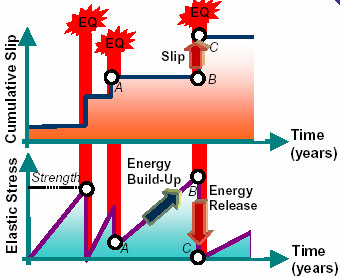
\includegraphics[height=3cm]{erb.png}
\caption{slip vs time and stress vs time}}
\end{figure}
  \end{itemize}
 
\end{frame}

\subsection{Tectonic Provinces in India}

\begin{frame}{Tectonic Provinces in India}
  The Indian landmass, covering an area of about 3.2 million sq km, has three broad morphotectonic provinces, namely
  \begin{itemize}
  \item Himalaya and Tertiary mobile belt
  \item Indo Gangetic Alluvial Plains
(IGAP)
  \item Peninsular shield
  \item Indo-Burma Arc
  \end{itemize}
  Peninsular India constitutes one of the most prominent
and largest Precambrian shield areas of the world. It is
exposed to the south of the IGAP, which separates the Himalayas
to the north and the peninsular India to the south.\\ While
the Himalaya is a region of dominant compressional
tectonics and the IGAP is a region of relatively less eventful
recent sedimentation, peninsular India, in contrast, is a
region marked by Early Archaean cratonisation with
associated Proterozoic belts; the cratons are separated by
‘rifts’.
\end{frame}

\begin{frame}
\begin{figure}
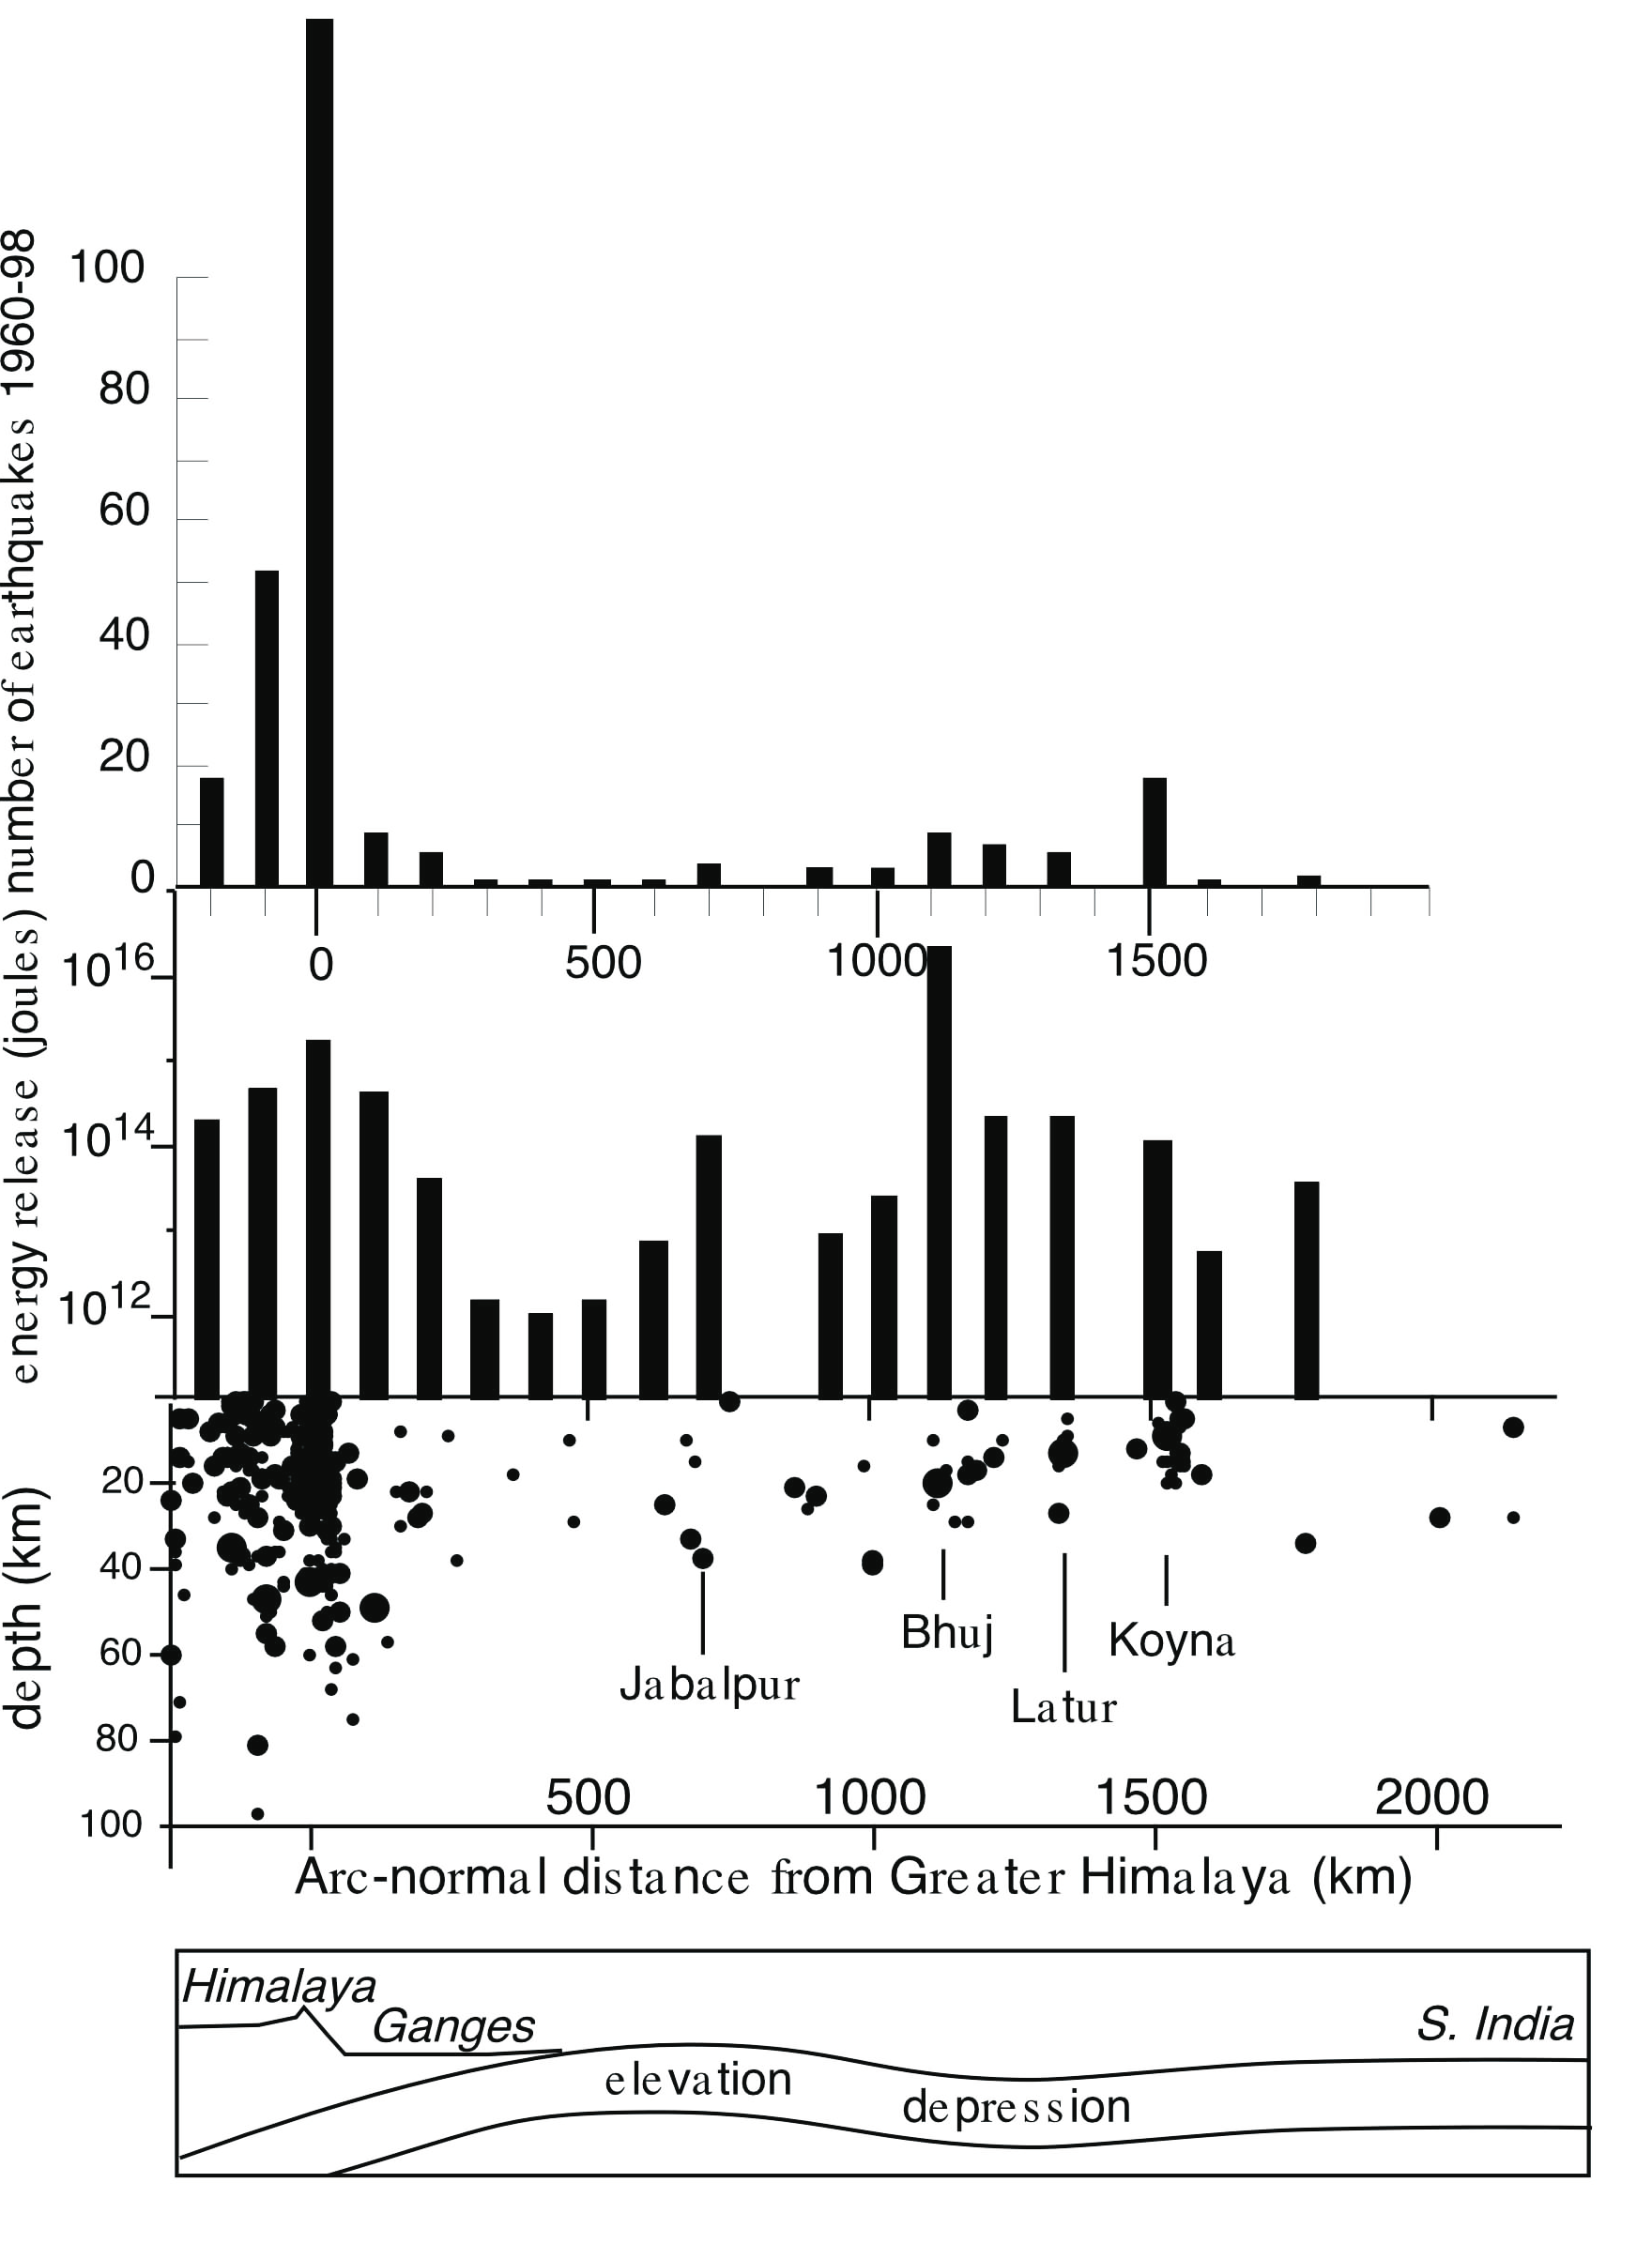
\includegraphics[height=5.1cm]{eqpd.png}
\caption{Seismic and structural sections through the Himalaya and Indian plate. Cumulative numbers of earthquakes since
1960, and their equivalent energy release, are binned in 100 km arc-normal distances. The locations of significant events are
named. Note the absence of seismicity below 40 km in the Indian plate.(\textit{Roger Bilham et al. 2003})}
\end{figure}
\end{frame}
\begin{frame}
	\begin{itemize}
	\item India is currently penetrating into Asia at a rate of approximately 45 mm/yr and rotating slowly anticlockwise
	 \begin{block}{Plate-Boundary}
The Himalaya marks the largest active continent-continent collision zone that has witnessed four great earthquakes in a short time span of 53 years between 1897
and 1950
\end{block}
	\begin{block}{Stable(relatively) Continenetal Region}
	The Peninsular India is a mosaic of Archaean nucleus with peripheral Proterozoic mobile belts, Cretaceous volcanism and rift-drift Mesozoic passive coastal basins.
\end{block}
	\item It was reported that the seismicity of peninsular India is low despite its ongoing collision with Central Asia (Chandra, 1977).
	\end{itemize}
\end{frame}
\section{Tectonic setting and related seismicity}

\subsection{The major thrust/fault systems of the Himalayan arc}


\begin{frame}{The major thrust/fault systems of the Himalayan arc}{spanning the entire
length from north to south, are:}
\begin{itemize}
	\item the Indus Suture Thrust (IST)
	\item the Main Central Thrust (MCT)
	\item the Main Boundary Thrust (MBT)
	\item the Himalayan Frontal Thrust (HFT)
\end{itemize}
\begin{block}{Main Himalayan Seismic Belt}
The seismicity between the MCT
and MBT is defined as the Main Himalayan Seismic Belt
(MHSB).
Many large (M>7.0) and great earthquakes
(M 8.0 and above) occurred in this belt.\\
During the last decade, two strong earthquakes
(M>6.0<7.0) occurred in the western Himalaya tectonic
zone, the 1991 Uttarkashi and the 1999 Chamoli
earthquakes and the 2005 Kashmir Earthquake.
\end{block}
\end{frame}
\subsection{Major prominent Rifts}
\begin{frame}{The major prominent Rifts}{hich separate the northern and southern blocks of the shield, are}
  \begin{block}{SONATA (Son-Narmada-Tapti Lineament) Zone}
	It is about 1000 km long and 50 km wide in the central part of India.
Three strong/large earthquakes (M 6.0~7.7) occurred in peninsular India: the 1993 Killari
earthquake in the southern block of the shield, the 1997
Jabalpur earthquake in the central SONATA zone
	\end{block}
	\begin{block}{Kutch rift}
	Kutch rift at the northwest at margin of the Indian shield has been plagued by the occurrence of the M 7.6 Bhuj 2001
earthquake less than two centuries after the 7.8 Allah Bund 1819 earthquake
	\end{block}
\end{frame}
\begin{frame}
\begin{figure}
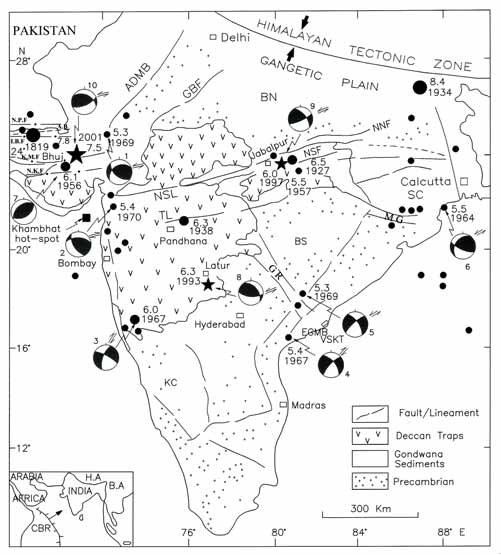
\includegraphics[height=6cm]{flmap.png}
\caption{Map showing seismotectonic domains in peninsular India and the signficant earthquakes with fault plane solutions, the three strong
earthquakes that occurred during the last decade are indicated by the star symbols}
\end{figure}
\end{frame}
\subsection{Regional  seismicity of the North-Eastern Region}
\begin{frame}{Regional  seismicity of the North-Eastern Region}
The high seismicity of the northeast Indian region
has been attributed to a complex tectonic province
displaying juxtaposition of the E–W trending
Himalaya and the N–S trending Arakan Yoma
belt.\\
The major tectonic background includes 
\begin{itemize}
\item the
eastern Himalayan structures, 
\item the Mishmi massif,
\item the Indo Myanmar arc, 
\item the Brahmaputra valley,
and \item the Shillong plateau.
\end{itemize}
The movement along the Po Chu fault, in the north-
eastern part of the region, is believed to have
caused the 1950 Great Assam Earthquake of M
8.7 (Ben-Menahem 1974; Thingbaijam et al 2008).
\end{frame}
\begin{frame}
\begin{figure}
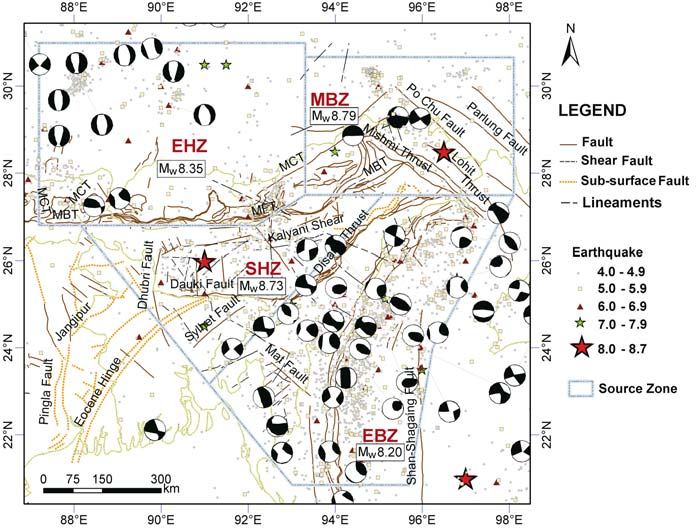
\includegraphics[height=6.5cm]{ne.png}
\caption{The four seismic source zones in the northeast Indian region}
\end{figure}
\end{frame}
% Placing a * after \section means it will not show in the
% outline or table of contents.
\section*{Summary}

\begin{frame}{Summary}
  \begin{itemize}
  \item
    The \alert{first main message} of your talk in one or two lines.
  \item
    The \alert{second main message} of your talk in one or two lines.
  \item
    Perhaps a \alert{third message}, but not more than that.
  \end{itemize}
  
  \begin{itemize}
  \item
    Outlook
    \begin{itemize}
    \item
      Something you haven't solved.
    \item
      Something else you haven't solved.
    \end{itemize}
  \end{itemize}
\end{frame}



% All of the following is optional and typically not needed. 
\appendix
\section<presentation>*{\appendixname}
\subsection<presentation>*{For Further Reading}

\begin{frame}[allowframebreaks]
  \frametitle<presentation>{For Further Reading}
    
  \begin{thebibliography}{10}
    
  \beamertemplatebookbibitems
  % Start with overview books.

  \bibitem{Author1990}
    A.~Author.
    \newblock {\em Handbook of Everything}.
    \newblock Some Press, 1990.
 
    
  \beamertemplatearticlebibitems
  % Followed by interesting articles. Keep the list short. 

  \bibitem{Someone2000}
    S.~Someone.
    \newblock On this and that.
    \newblock {\em Journal of This and That}, 2(1):50--100,
    2000.
  \end{thebibliography}
\end{frame}

\end{document}


